\begin{name}
	{\tenchude}
	{TOÁN 10}
	{LỚP TOÁN THẦY PHÁT}
	{Thời gian: 90 phút - Không kể thời gian phát đề}
\end{name}
\noindent{\bf\fontfamily{qag}\selectfont\color{violet}A. PHẦN TRẮC NGHIỆM}
\Opensolutionfile{ans}[ans/ans-0-GK1-CTST-De10-NH23-24]
\begin{ex}%[0-GK1-NH22-23--TeamTeXHoa--Võ Thị Thùy Trang]%[0T1Y1-1]
	Trong các khẳng định sau, có bao nhiêu khẳng định là mệnh đề?
	\begin{enumerate}
		\item[(I):] \lq\lq $2+4=7$\rq\rq.
		\item[(II):] \lq\lq$3x-1=0$\rq\rq.
		\item[(III):] \lq\lq Hình vuông là tứ giác có bốn góc vuông và bốn cạnh bằng nhau\rq\rq.
		\item[(IV):] \lq\lq$3$ là số lẻ\rq\rq.
	\end{enumerate}
	\choice
	{$1$}
	{\True $3$}
	{$2$}
	{$4$}
	\loigiai{
		Các khẳng định (I), (III), (IV) là mệnh đề.	
	}
\end{ex}
%Câu 2
\begin{ex}%[0-GK1-NH22-23--TeamTeXHoa--Võ Thị Thùy Trang]%[0T1Y1-3]
	Cho mệnh đề $A\colon$\lq\lq$\forall x \in \mathbb{R}\colon x^2+1>0$\rq\rq. Trong các mệnh đề sau, mệnh đề nào là phủ định của mệnh đề $A$?
	\choice
	{$\overline{A}\colon$\lq\lq$\exists x\in \mathbb{R}\colon x^2+1>0$\rq\rq}
	{$\overline{A}\colon$\lq\lq$\forall x\in \mathbb{R}\colon x^2+1 \leq 0$\rq\rq}
	{$\overline{A}\colon$\lq\lq$\forall x\in \mathbb{R}\colon x^2+1 \neq 0$\rq\rq}
	{\True $\overline{A}\colon $\lq\lq$\exists x\in \mathbb{R}\colon x^2+1 \leq 0$\rq\rq}
	\loigiai{
		Mệnh đề phủ định $\overline{A}\colon$\lq\lq$\exists x\in \mathbb{R}\colon x^2+1 \leq 0$\rq\rq.	
	}
\end{ex}
%Câu 3
\begin{ex}%[0-GK1-NH22-23--TeamTeXHoa--Võ Thị Thùy Trang]%[0T1Y2-1]
	Cho tập hợp $A=\{x\in \mathbb{Z} \Big| -3<x \leq 4\}$. Khẳng định nào sau đây đúng?
	\choice
	{\True $A=\{-2;-1;0;1;2;3;4\}$}
	{$A=\left(-3;4\right]$}
	{$A=\{-2;-1;0;1;2;3\}$}
	{$A=\{-3;-2;-1;0;1;2;3;4\}$}
	\loigiai{
		Ta có tập hợp $A=\{-2;-1;0;1;2;3;4\}$. 	
	}
\end{ex}
%Câu 4
\begin{ex}%[0-GK1-NH22-23--TeamTeXHoa--Võ Thị Thùy Trang]%[0T1B3-5]
	Cho hai tập hợp $A=\left(1;5\right]$; $B=\left(2;7\right]$. Tập hợp $A \setminus B$ là
	\choice
	{\True $\left(1;2\right]$}
	{$\left(2;5\right)$}
	{$\left(-1;7\right]$}
	{$\left(-1;2\right)$}
	\loigiai{
		Ta có $A \setminus B=\left(1;2\right]$. 	
	}
\end{ex}
%Câu 5
\begin{ex}%[0-GK1-NH22-23--TeamTeXHoa--Võ Thị Thùy Trang]%[0T1B2-2]
	Cho tập hợp $A=\{a;b;1;2;3\}$. Số tập con gồm hai phần tử của tập $A$ là
	\choice
	{$20$}
	{\True $10$}
	{$12$}
	{$15$}
	\loigiai{
		Các tập con gồm hai phần tử của tập $A$ là\\
		$\{a;b\}, \{a;1\}, \{a;2\}, \{a;3\}, \{b;1\}, \{b;2\}, \{b;3\}, \{1;2\}, \{1;3\}, \{2;3\}$.\\
		Vậy có $10$ tập con gồm hai phần tử của tập $A$.	
	}
\end{ex}
%Câu 6
\begin{ex}%[0-GK1-NH22-23--TeamTeXHoa--Võ Thị Thùy Trang]%[0T1B3-4]
	Cho các tập hợp $A=\left[-5;\dfrac{1}{2}\right]$, $B=\left(-3;+\infty\right)$. Khi đó tập hợp $A \cap B$ bằng
	\choice
	{$\left\{x\in \mathbb{R} \Big| -3 \leq x \leq \dfrac{1}{2}\right\}$}
	{\True $\left\{x\in \mathbb{R} \Big| -3<x \leq \dfrac{1}{2}\right\}$}
	{$\left\{x\in \mathbb{R} \Big| -5<x \leq \dfrac{1}{2}\right\}$}
	{$\left\{x\in \mathbb{R} \Big| -3 \leq x < \dfrac{1}{2}\right\}$}
	\loigiai{
		Ta có $A \cap B=\left(-3;\dfrac{1}{2}\right]=\{x\in \mathbb{R} \Big| -3<x \leq \dfrac{1}{2}\}$.\\
	}
\end{ex}
%Câu 7
\begin{ex}%[0-GK1-NH22-23--TeamTeXHoa--Võ Thị Thùy Trang]%[0T2Y1-1]
	Bất phương trình nào sau đây là bất phương trình bậc nhất hai ẩn?
	\choice
	{$2x^2+3y^2<0$}
	{$2x^2-y>0$}
	{$2x+3y^2>0$}
	{\True $2x+3y<0$}
	\loigiai{
		Bất phương trình $2x+3y<0$ là bất phương trình bậc nhất hai ẩn. Các bất phương trình còn lại không phải là bất phương trình bậc nhất hai ẩn vì có chứa $x^2$, $y^2$. 	
	}
\end{ex}
%Câu 8
\begin{ex}%[0-GK1-NH22-23--TeamTeXHoa--Võ Thị Thùy Trang]%[0T2Y1-1]
	Điểm nào sau đây thuộc miền nghiệm của bất phương trình $x+5y-3<0$?
	\choice
	{$M(1;2)$}
	{$N(-1;7)$}
	{$P(0;2)$}
	{\True $Q(-8;1)$}
	\loigiai{
		Ta thấy cặp số $(-8;1)$ thoả mãn bất phương trình $x+5y-3<0$ nên điểm $Q(-8;1)$ thuộc miền nghiệm của bất phương trình $x+5y-3<0$.	
	}
\end{ex}
%Câu 9
\begin{ex}%[0-GK1-NH22-23--TeamTeXHoa--Võ Thị Thùy Trang]%[0T2Y2-1]
	Điểm $O(0;0)$ thuộc miền nghiệm của hệ bất phương trình nào sau đây?
	\choice
	{$ \left\{\begin{aligned}
			&x+3y-6>0\\
			&2x+y+4>0\\
		\end{aligned}\right.$}
	{$ \left\{\begin{aligned}
			&x+3y-6>0\\
			&2x+y+4<0\\
		\end{aligned}\right.$}
	{\True $ \left\{\begin{aligned}
			&x+3y-6<0\\
			&2x+y+4>0\\
		\end{aligned}\right.$}
	{$ \left\{\begin{aligned}
			&x+3y-6<0\\
			&2x+y+4<0\\
		\end{aligned}\right.$}
	\loigiai{
		Thay cặp số $O(0;0)$ vào các hệ bất phương trình ta được đáp án.	
	}
\end{ex}
%Câu 10
\begin{ex}%[0-GK1-NH22-23--TeamTeXHoa--Võ Thị Thùy Trang]%[0T2Y2-1]
	Cặp số nào sau đây là nghiệm của hệ bất phương trình $ \left\{\begin{aligned}
		&x-2y \leq 8\\
		&3x+y>3\\
	\end{aligned}\right.$
	\choice
	{$(0;1)$}
	{$(0;-4)$}
	{$(1;-1)$}
	{\True $(1;1)$}
	\loigiai{
		Lần lượt thay các bộ số ở các phương án vào hệ bất phương trình ta được một nghiệm của hệ bất phương trình trên là $(1;1)$. 	
	}
\end{ex}
%Câu 11
\begin{ex}%[0-GK1-NH22-23--TeamTeXHoa--Võ Thị Thùy Trang]%[0T2Y2-1]
	Tìm hệ bất phương trình bậc nhất hai ẩn trong các hệ sau
	\choice
	{$ \left\{\begin{aligned}
			&2x+y-5=0\\
			&3x-4y-10=0\\
		\end{aligned}\right.$}
	{\True $ \left\{\begin{aligned}
			&x-y-4<0\\
			&3x+2y-6<0\\
		\end{aligned}\right.$}
	{$ \left\{\begin{aligned}
			&x^2-3x-3 \leq 0\\
			&x+4y-5<0\\
		\end{aligned}\right.$}
	{$ \left\{\begin{aligned}
			&x+y-7>0\\
			&3x-y^2-5<0\\
		\end{aligned}\right.$}
	\loigiai{
		Hệ bất phương trình bậc nhất hai ẩn là $ \left\{\begin{aligned}
			&x-y-4<0\\
			&3x+2y-6<0\\
		\end{aligned}\right.$.	
	}
\end{ex}
%Câu 12
\begin{ex}%[0-GK1-NH22-23--TeamTeXHoa--Võ Thị Thùy Trang]%[0T2B2-1]
	Cho hệ bất phương trình bậc nhất hai ẩn $ \left\{\begin{aligned}
		&x+y-5>0\\
		&2x-3y-20<0\\
	\end{aligned}\right.$ có tập nghiệm $S$. Khẳng định nào sau đây đúng?
	\choice
	{\True $(1;5) \in S$}
	{$(1;2) \in S$}
	{$(2;-4) \in S$}
	{$(5;-2) \in S$}
	\loigiai{
		Vì $1+5-5=1>0$ và $2 \cdot 1 -3 \cdot 5 -20=-33<0$ nên $(1;5)$ là nghiệm của hệ bất phương trình $ \left\{\begin{aligned}
			&x+y-5>0\\
			&2x-3y-20<0\\
		\end{aligned}\right.$. 
	}
\end{ex}
%Câu 13
\begin{ex}%[0-GK1-NH22-23--TeamTeXHoa--Võ Thị Thùy Trang]%[0T4Y1-2]
	Giá trị của biểu thức $A=4 \cos 60^{\circ}+2\sin 30^{\circ}-3\tan 45^{\circ}$ bằng	
	\choice
	{$\dfrac{1}{2}$}
	{\True $0$}
	{$\dfrac{1}{4}$}
	{$2$}
	\loigiai{
		Ta có $A=4 \cos 60^{\circ}+2\sin 30^{\circ}-3\tan 45^{\circ}=4 \cdot \dfrac{1}{2} + 2\cdot \dfrac{1}{2}-3 \cdot 1=0$ 	
	}
\end{ex}
%Câu 14
\begin{ex}%[0-GK1-NH22-23--TeamTeXHoa--Võ Thị Thùy Trang]%[0T4Y1-1]
	Cho $\cos \alpha=\sqrt{1-\sin^2\alpha}$. Khẳng định nào sau đây đúng?	
	\choice
	{$90^{\circ}<\alpha<180^{\circ}$}
	{\True $0^{\circ} \leq \alpha \leq 90^{\circ}$}
	{$0^{\circ} \leq \alpha \leq 180^{\circ}$}
	{$0^{\circ}<\alpha<180^{\circ}$}
	\loigiai{
		Ta có $\cos \alpha=\sqrt{1-\sin^2\alpha}=\sqrt{\cos^2\alpha}=\left|\cos \alpha\right|  \Leftrightarrow \cos \alpha \ge 0 \Leftrightarrow 0^{\circ} \leq \alpha \leq 90^{\circ}$.	
	}
\end{ex}
%Câu 15
\begin{ex}%[0-GK1-NH22-23--TeamTeXHoa--Võ Thị Thùy Trang]%[0T4Y1-1]
	Trên nửa đường tròn đơn vị có hai điểm $M, M'$ đối xứng nhau qua trục tung; gọi các góc $\alpha=\widehat{xOM}, \beta =\widehat{xOM'}$ (như hình vẽ).\\
	\begin{center}
		\begin{tikzpicture}[scale=0.8,>=stealth, font=\footnotesize, line join=round, line cap=round]
			\draw[->] (-4,0)--(4,0) node [below]{$x$};
			\draw[->] (0,-1)--(0,4) node [right]{$y$};
			\draw (-3,0) arc (180:0:3);
			\coordinate(O)(0,0);
			\coordinate(M')(-2.59,1.5);
			\coordinate(M)(2.59,1.5);
			\draw (-2.59,1.5) node [above left]{$M'$} (2.59,1.5) node [above right]{$M$};
			\draw (-3,0) node [below]{$A'$} (3,0) node [below]{$A$} (0,3) node [above right]{$B$} (0,1.5) node [above right]{$H$};
			\draw[dashed] (-4,1.5)--(4,1.5);
			\draw (O) node [below left]{$O$} --(M) (O)--(M');
			\draw (M') circle (1pt) (M) circle (1pt);
		\end{tikzpicture}
	\end{center}
	Hỏi mối liên hệ giữa hai góc $\alpha, \beta$ là gì?
	\choice
	{Phụ nhau}
	{\True Bù nhau}
	{Bằng nhau}
	{Hơn kém nhau $90^{\circ}$}
	\loigiai{
		Ta có $M,M'$ đối xứng nhau qua trục tung và $A,A'$ đối xứng nhau qua trục tung nên $AM=A'M'  \Rightarrow \widehat{AOM}=\widehat{A'OM'}$.\\
		Ta có: $\widehat{AOM'}+\widehat{MOA}=\widehat{AOM'}+\widehat{M'OA'}=\widehat{AOA'}=180^{\circ}$.\\
		Vậy $\alpha, \beta$ là hai góc bù nhau.	
	}
\end{ex}
\begin{ex}%[0-GK1-NH22-23--TeamTeXHoa--Võ Thị Thùy Trang]%[0T4B2-1]
	Khăn quàng đội viên có hình tam giác cân với kích thước như trong hình vẽ. Góc lớn nhất của tam giác cân gần nhất với số đo nào?
	\begin{center}
		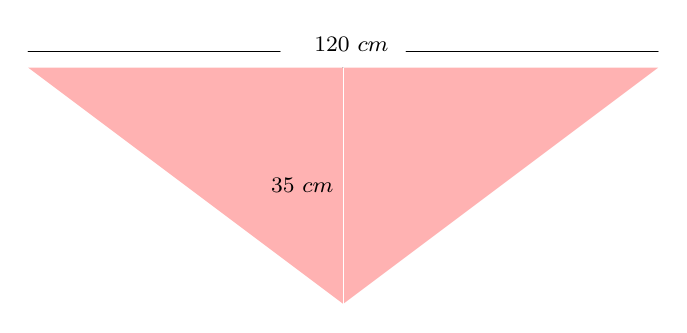
\begin{tikzpicture}[>=stealth, font=\footnotesize, line join=round, line cap=round]
			\coordinate(H) (0,0);
			\coordinate(A) (-4,0);
			\coordinate(B) (4,0);
			\coordinate(C) (0,-3);
			\fill[red!30] (-4,0)--(0,-3)--(4,0)--cycle;
			\draw (0.7,0.3) node [left]{$120 \ \text{cm}$} (0,-1.5) node [left]{$35 \ \text{cm}$};
			\draw (C)--(H);
			\draw (-4,0.2)--(-0.8,0.2) (0.8,0.2)--(4,0.2);
			\draw[white] (0,0)--(0,-3);
		\end{tikzpicture}
	\end{center}
	\choice
	{$90^{\circ}$}
	{\True $120^{\circ}$}
	{$135^{\circ}$}
	{$150^{\circ}$}
	\loigiai{
		Đặt các đỉnh của hình tam giác như hình vẽ.
		\begin{center}
			\begin{tikzpicture}[>=stealth, font=\footnotesize, line join=round, line cap=round]
				\coordinate(H) (0,0);
				\coordinate(A) (-4,0);
				\coordinate(B) (4,0);
				\coordinate(C) (0,-3);
				\draw (0,0)--(0,-3);
				\draw (-4,0)--(0,-3)--(4,0)--cycle;%\fill[red] 
				\draw (-4,0) node [left]{$A$} (4,0) node [right]{$B$} (0,-3) node [below]{$C$} (0,0) node [below right]{$H$} (0.7,0.3) node [left]{$120 \ \text{cm}$} (0,-1.5) node [left]{$35 \ \text{cm}$};
				\draw (A) circle (1pt) (B) circle (1pt) (C) circle (1pt) (H) circle (1pt);
				\draw (-4,0.2)--(-0.8,0.2) (0.8,0.2)--(4,0.2);
			\end{tikzpicture}
		\end{center}
		Khi đó $\tan \widehat{HCB}=\dfrac{BH}{CH}=\dfrac{12}{7} \Rightarrow \widehat{HCB} \approx 59,7^{\circ} \Rightarrow \widehat{ACB} \approx 119{,}4^{\circ}$.\\
		Vậy chọn $\widehat{ACB} \approx 120^{\circ}$.	
	}
\end{ex}
\begin{ex}%[0-GK1-NH22-23--TeamTeXHoa--Võ Thị Thùy Trang]%[0H1B2-1]
	Cho tam giác $ABC$ có $AB=14$cm, $AC=10$cm và $BC=16$cm. Tính góc $C$ của tam giác $ABC$.
	\choice
	{$30^{\circ}$}
	{$45^{\circ}$}
	{\True $60^{\circ}$}
	{$120^{\circ}$}
	\loigiai{
		Ta có $\cos C=\dfrac{AC^2+BC^2-AB^2}{2 \cdot AC \cdot BC}=\dfrac{10^2+16^2-14^2}{2 \cdot 10 \cdot 16}=\dfrac{1}{2} \Rightarrow \widehat{C}=60^{\circ}$.	
	}
\end{ex}

%Câu 18
\begin{ex}%[0-GK1-NH22-23--TeamTeXHoa--Võ Thị Thùy Trang]%[0H1B2-1]
	Cho tam giác $ABC$ có $a=3$, $b=5$, $c=7$. Tính $S=\sin A-2\sin B+\sin C$.
	\choice
	{\True $0$}
	{$1$}
	{$2$}
	{$-1$}
	\loigiai{
		Ta có $S=\sin A-2\sin B+\sin C=\dfrac{a}{2R}-2 \cdot \dfrac{b}{2R}+ \dfrac{c}{2R}=\dfrac{a-2b+c}{2R}=\dfrac{3-2 \cdot 5+7}{2R}=0$.	
	}
\end{ex}
\begin{ex}%[0-GK1-NH22-23--TeamTeXHoa--Võ Thị Thùy Trang]%[0T4Y2-1]
	Cho tam giác $ABC$ có $a=5$, $\widehat{A}=60^{\circ}$. Tính bán kính đường tròng ngoại tiếp tam giác $ABC$.
	\choice
	{$\dfrac{10\sqrt{3}}{3}$}
	{$\dfrac{5}{3}$}
	{$5\sqrt{3}$}
	{\True $\dfrac{5\sqrt{3}}{3}$}
	\loigiai{
		Theo định lí sin ta có $R=\dfrac{a}{2\sin A}=\dfrac{5}{2 \cdot \sin60^{\circ}}=\dfrac{5\sqrt{3}}{3}$.	
	}
\end{ex}
%Câu 20
\begin{ex}%[0-GK1-NH22-23--TeamTeXHoa--Võ Thị Thùy Trang]%[0T4Y2-2]
	Tính diện tích tam giác $ABC$ biết $b=2$, $c=5$, $\widehat{A}=30^{\circ}$.
	\choice
	{$10$}
	{$5$}
	{\True $\dfrac{5}{2}$}
	{$5\sqrt{3}$}
	\loigiai{
		Diện tích tam giác $ABC$ là $S=\dfrac{1}{2}bc\sin A=\dfrac{1}{2} \cdot 2 \cdot 5 \cdot \sin 30^{\circ}=\dfrac{5}{2}$.	
	}
\end{ex}
\begin{ex}%[0-GK1-NH22-23--TeamTeXHoa--Võ Thị Thùy Trang]%[0T1B1-2]
	Trong các mệnh đề sau, mệnh đề nào là mệnh đề \textbf{sai}?
	\choice
	{$\exists x\in \mathbb{Z},2x^2-8=0$}
	{$\pi <5\Leftrightarrow{\pi^2}<25$}
	{$7<3\Rightarrow 9>5$}
	{\True $\forall x\in \mathbb{R},\left(x-4\right)^2<x^2+3$}
	\loigiai{
		Với $x=2$ thì $2x^2-8=0$ nên mệnh đề \lq\lq $\exists x\in \mathbb{Z},2x^2-8=0$\rq\rq~ là đúng.\\
		Ta có mệnh đề \lq\lq $\pi <5$\rq\rq~ và mệnh đề \lq\lq $\pi^2<25$\rq\rq~ là mệnh đề đúng nên mệnh đề \lq\lq$\pi <5\Leftrightarrow{\pi^2}<25$\rq\rq~ là mệnh đề đúng. Vậy $\pi <5\Leftrightarrow{\pi^2}<25$ đúng.\\
		Ta có mệnh đề \lq\lq $7<3$\rq\rq~ là mệnh đề sai và mệnh đề \lq\lq $9>5$\rq\rq là mệnh đề đúng nên mệnh đề \lq\lq $7<3\Rightarrow 9>5$\rq\rq~ là mệnh đề đúng. Vậy $7<3\Rightarrow 9>5$ đúng.\\
		Với $x=-1\in \mathbb{R}$ thì $\left(x-4\right)^2=25$; $x^2+3=4$ nên mệnh đề \lq\lq $\forall x\in \mathbb{R},\left(x-4\right)^2<x^2+3$\rq\rq~  là mệnh đề sai.}
\end{ex}
\begin{ex}%[0-GK1-NH22-23--TeamTeXHoa--Võ Thị Thùy Trang]%[0T1B1-3]
	Lập mệnh đề phủ định của mệnh đề \lq\lq$\forall x\in \mathbb{R}\colon x^2+x+2022>0$\rq\rq.
	\choice
	{$\forall x\in \mathbb{R}\colon x^2+x+2022<0$}
	{$\forall x\in \mathbb{R}\colon x^2+x+2022\le 0$}
	{$\exists x\in \mathbb{R}\colon x^2+x+2022<0$}
	{\True $\exists x\in \mathbb{R}\colon x^2+x+2022\le 0$}
	\loigiai{
		Mệnh đề phủ định của mệnh đề \lq\lq $\forall x\in \mathbb{R}\colon x^2+x+2022>0$\rq\rq ~là mệnh đề \lq\lq $\exists x\in \mathbb{R}\colon x^2+x+2022\le 0$\rq\rq.}
\end{ex}
\begin{ex}%[0-GK1-NH22-23--TeamTeXHoa--Võ Thị Thùy Trang]%[0T1B3-1]
	Cho hai tập $A=\left\{x\in \mathbb{R}\Big|3x+3>5+x\right\}$, $B=\left\{x\in \mathbb{R}\Big|5x-7<4x-1\right\}$. Tất cả các số tự nhiên thuộc cả hai tập $A$ và $B$ là
	\choice
	{$\left\{2;3;4;5;6\right\}$}
	{$\left\{1;2;3;4;5;6\right\}$}
	{\True $\left\{2;3;4;5\right\}$}
	{Không có}
	\loigiai{
		$A=\left\{x\in \mathbb{R}\Big|3x+3>5+x\right\}\Rightarrow A=\left(1;+\infty\right)$\\
		$B=\left\{x\in \mathbb{R}\Big|5x-7<4x-1\right\}\Rightarrow B=\left(-\infty;6\right)$\\
		$A\cap B=\left(1;6\right)\Leftrightarrow A\cap B=\left\{x\in \mathbb{R}\Big|1<x<6\right\}$.\\
		$\Rightarrow A\cap B=\left\{x\in \mathbb{N}\Big|1<x<6\right\}\Leftrightarrow A\cap B=\left\{2;3;4;5\right\}$.}
\end{ex}
\begin{ex}%[0-GK1-NH22-23--TeamTeXHoa--Võ Thị Thùy Trang]%%[0T1B2-1]
	Trong các tập sau, tập nào là tập rỗng?
	\choice
	{$\left\{x\in \mathbb{N}\Big|\left| x\right|<2\right\}$}
	{$\left\{x\in \mathbb{Z}\Big|3x^2-2x-1=0\right\}$}
	{\True $\left\{x\in \mathbb{Q}\Big|x^2-4x+1=0\right\}$}
	{$\left\{x\in \mathbb{R}\Big|x^2-4x+3=0\right\}$}
	\loigiai{
		$A=\left\{x\in \mathbb{N}\Big|\left| x\right|<2\right\}\Rightarrow A=\left\{0;1\right\}$.\\
		$B=\left\{x\in \mathbb{Z}\Big|3x^2-2x-1=0\right\}\Rightarrow B=\left\{1\right\}$.\\
		$C=\left\{x\in \mathbb{Q}\Big|x^2-4x+1=0\right\}\Rightarrow C=\varnothing $.\\
		$D=\left\{x\in \mathbb{R}\Big|x^2-4x+3=0\right\}\Rightarrow D=\left\{1;3\right\}$.}
\end{ex}
\begin{ex}%[0-GK1-NH22-23--TeamTeXHoa--Võ Thị Thùy Trang]%[0T1B3-2]
	Cho các tập hợp $A=\left\{x\in \mathbb{N}\Big| x^2-3x=0\right\}$, $B=\left\{0;1;2;3\right\}$. Tập $B\setminus A$ bằng
	\choice
	{\True $\left\{1;2\right\}$}
	{$\left\{5;6\right\}$}
	{$\left\{0\right\}$}
	{$\left\{0;1\right\}$}
	\loigiai{
		Ta có $x^2-3x=0\Leftrightarrow \left[\begin{matrix}
			x=3 \\
			x=0 \\
		\end{matrix}\right.$ nên $A=\left\{x\in \mathbb{N}\Big|x^2-3x=0\right\}=\left\{0;3\right\}$.\\
		Theo định nghĩa $x\in B\setminus A\Leftrightarrow \left[\begin{matrix}
			x\in B \\
			x\notin A \\
		\end{matrix}\right.$ nên $B\setminus A=\left\{1;2\right\}$.}
\end{ex}
\begin{ex}%[0-GK1-NH22-23--TeamTeXHoa--Võ Thị Thùy Trang]%[0T2B1-2]
	Biểu diễn hình học của tập nghiệm của bất phương trình $2x+y\ge 1$ là
	\choice
	{\True \begin{tikzpicture}[>=stealth,x=1cm,y=1cm,scale=.5]
			\draw[->] (-4,0)--(4,0)node[below right]{$x$};
			\draw[->] (0,-4)--(0,4) node[left]{$y$};
			\draw (0,0)node[below left]{$O$};
			\path[pattern = north east lines] (-1.5,4)-|(-4,-4)--(2.5,-4)--cycle;
			\draw (-1.5,4)--(2.5,-4);
			\fill[black] (1/2,0)circle(1pt);
			\coordinate[label=above right:\tiny{$\frac{1}{2}$}] ()at(1/2,0);
			\coordinate[label=right:\tiny{$1$}] ()at(0,1);
			\fill[black] (0,1)circle(1pt);	
	\end{tikzpicture} }
	{\begin{tikzpicture}[>=stealth,x=1cm,y=1cm,scale=.5]
			\draw[->] (-4,0)--(4,0)node[below right]{$x$};
			\draw[->] (0,-4)--(0,4) node[left]{$y$};
			\draw (0,0)node[below left]{$O$};
			\path[pattern = north east lines] (-1.5,4)-|(4,-4)--(2.5,-4)--cycle;
			\draw (-1.5,4)--(2.5,-4);
			\fill[black] (1/2,0)circle(1pt);
			\coordinate[label=below:\tiny{$\frac{1}{2}$}] ()at(1/2,0);
			\coordinate[label=left:\tiny{$1$}] ()at(0,1);
			\fill[black] (0,1)circle(1pt);	
	\end{tikzpicture}}
	{\begin{tikzpicture}[>=stealth,x=1cm,y=1cm,scale=.5]
			\draw[->] (-4,0)--(4,0)node[below right]{$x$};
			\draw[->] (0,-4)--(0,4) node[left]{$y$};
			\draw (0,0)node[below left]{$O$};
			\path[pattern = north east lines] (-4,2.5)|-(4,-4)--(4,-1.5)--cycle;
			\draw (-4,2.5)--(4,-1.5);
			\fill[black] (0,1/2)circle(1pt);
			\coordinate[label=right:\tiny{$\frac{1}{2}$}] ()at(0,1/2);
			\coordinate[label=above:\tiny{$1$}] ()at(1,0);
			\fill[black] (1,0)circle(1pt);	
	\end{tikzpicture}}
	{\begin{tikzpicture}[>=stealth,x=1cm,y=1cm,scale=.5]
			\draw[->] (-4,0)--(4,0)node[below right]{$x$};
			\draw[->] (0,-4)--(0,4) node[left]{$y$};
			\draw (0,0)node[below left]{$O$};
			\path[pattern = north east lines] (-4,2.5)|-(4,4)--(4,-1.5)--cycle;
			\draw (-4,2.5)--(4,-1.5);
			\fill[black] (0,1/2)circle(1pt);
			\coordinate[label=left:\tiny{$\frac{1}{2}$}] ()at(0,1/2);
			\coordinate[label=below:\tiny{$1$}] ()at(1,0);
			\fill[black] (1,0)circle(1pt);
	\end{tikzpicture}}
	\loigiai{
		Đường thẳng $d\colon 2x+y=1$ đi qua hai điểm $\left(0;1\right)$ và $\left(\dfrac{1}{2};0\right)$.\\
		Xét điểm $O\left(0;0\right)$ có $2.0+0\le 1$. Do đó miền nghiệm của bất phương trình là nửa mặt phẳng bờ là đường thẳng $d$, không chứa gốc $O$.
	}
\end{ex}
\begin{ex}%[0-GK1-NH22-23--TeamTeXHoa--Võ Thị Thùy Trang]%[0T2B1-2]
	\immini{
		Phần không tô dậm trong hình vẽ biểu diễn tập nghiệm của bất phương trình nào trong các bất phương trình sau?
		\choice
		{$2x-y>3$}
		{$x-2y<3$}
		{$x-2y>3$}
		{\True $2x-y<3$}
	}
	{\begin{tikzpicture}[>=stealth,x=1cm,y=1cm,scale=.5]
			\draw[->] (-4,0)--(4,0)node[below right]{$x$};
			\draw[->] (0,-4)--(0,4) node[left]{$y$};
			\draw (0,0)node[below left]{$O$};
			\path[pattern = north east lines] (-0.5,-4)-|(4,4)--(3.5,4)--cycle;
			\draw (-0.5,-4)--(3.5,4);
			\fill[black] (0,-3)circle(1pt);
			\coordinate[label=left:$-3$] ()at(0,-3);
			\coordinate[label=above:\tiny{$\tfrac{3}{2}$}] ()at(3/2,0);
			\fill[black] (3/2,0)circle(1pt);
	\end{tikzpicture}}
	\loigiai{
		Nhận xét: Miền nghiệm là phần chứa điểm $O\left(0;0\right)$ nên loại phương án $x-2y>3$ và $2x-y>3$.\\
		Đường thẳng $d\colon 2x-y=3$ cắt trục $Ox$ tại $A\left(\dfrac{3}{2};0\right)$, cắt trục $Oy$ tại $B\left(0;-3\right)$ nên chọn đáp án $2x-y<3$.}
\end{ex}
\begin{ex}%[0-GK1-NH22-23--TeamTeXHoa--Võ Thị Thùy Trang]%[0T2B2-2]
	Điểm $M\left(x;y\right)$ là điểm có tung độ nhỏ nhất thuộc miền nghiệm của hệ bất phương trình $\heva{&2x+y\le 1\\&x-y\le 2\\&5x+y\ge -4}$. Tính $F=y-x$.
	\choice
	{$-8$}
	{$2$}
	{\True $-2$}
	{$8$}
	\loigiai{
		Miền nghiệm của hệ bất phương trình $\heva{&2x+y\le 1\\&x-y\le 2\\&5x+y\ge -4}$ trên hệ trục toạ độ $Oxy$ là phần không bị xoá kể cả biên như hình vẽ.	
		\begin{center}
			\begin{tikzpicture}[>=stealth,x=1cm,y=1cm,scale=1]
				\draw[->] (-4,0)--(4,0)node[below right]{$x$};
				\draw[->] (0,-4)--(0,7) node[left]{$y$};
				\draw (0,0)node[below right]{$O$};
				\path[fill=blue!40] (-2.5,7)-|(4,-4)--(3,-4)--cycle;
				\draw (-2.5,7)--(3,-4);
				\path[pattern=crosshatch dots] (-2,-4)-|(4,2)--cycle;
				\draw (-2,-4)--(4,2);
				\path[pattern=crosshatch dots] (-2.20,7)-|(-4,-4)--(0,-4)--cycle;
				\draw (-2.20,7)--(0,-4);
				\fill[black] (0,-7/3)circle(1pt);
				\coordinate[label= above right:\tiny{$-\tfrac{7}{3}$}] ()at(0,-7/3);
				\coordinate[label=above:\small{$-\tfrac{1}{3}$}] ()at(-1/3,0);
				\fill[black] (-1/3,0)circle(1pt);
				\fill[black] (-1/3,-7/3)circle(1pt);
				\draw[dashed] (-1/3,0)--(-1/3,-7/3)--(0,-7/3);
			\end{tikzpicture}
		\end{center}
		Dựa vào hình vẽ ta có điểm có tung độ nhỏ nhất thuộc miền nghiêm của hệ bất phương trình là điểm $B\left(-\dfrac{1}{3};-\dfrac{7}{3}\right)$.\\
		Khi đó $F=y-x=\dfrac{-7}{3}-\left(\dfrac{-1}{3}\right)=-2$.}
\end{ex}
\begin{ex}%[0-GK1-NH22-23--TeamTeXHoa--Võ Thị Thùy Trang]%[0T2Y2-1]
	Điểm nào sau dây thuộc miền nghiệm của hệ bất phương trình $\heva{&2x+y-6<0\\&x-3y+5>0\\&x+1>0}$?
	\choice
	{$M\left(-;7\right)$}
	{\True $N\left(1;1\right)$}
	{$P\left(2;3\right)$}
	{$Q\left(-1;2\right)$}
	\loigiai{
		Ta thấy $N\left(1;1\right)$ thoả mãn hệ bất phương trình đã cho.}
\end{ex}
\begin{ex}%[0-GK1-NH22-23--TeamTeXHoa--Võ Thị Thùy Trang]%[0T4B1-2]
	Biết $\sin \alpha =\dfrac{2}{5}~\left(90^\circ<\alpha <180^\circ\right)$. Hỏi giá trị $\tan \alpha $ là bao nhiêu?
	\choice
	{\True $-\dfrac{2\sqrt{2}}{21}$}
	{$\dfrac{2\sqrt{2}}{21}$}
	{$2$}
	{$-2$}
	\loigiai{
		Vì $90^\circ<\alpha <180^\circ\Rightarrow \cos \alpha <0\Rightarrow \cos \alpha =-\sqrt{1-\sin^2\alpha}=-\sqrt{1-\dfrac{4}{25}}=-\dfrac{\sqrt{21}}{5}$.\\
		Vậy $\tan \alpha =\dfrac{\sin \alpha}{\cos \alpha}=-\dfrac{2\sqrt{21}}{21}$.}
\end{ex}
\begin{ex}%[0-GK1-NH22-23--TeamTeXHoa--Võ Thị Thùy Trang]%[0T4B1-2]
	Cho $\alpha $ là góc tù và $\sin \alpha =\dfrac{5}{13}$. Giá trị của biểu thức $3\sin \alpha +2\cos \alpha $ là
	\choice
	{$\dfrac{9}{13}$}
	{$3$}
	{\True $-\dfrac{9}{13}$}
	{$-3$}
	\loigiai{
		Ta có $\cos^2\alpha =1-\sin^2\alpha \Leftrightarrow{\cos^2}\alpha= \dfrac{144}{169}$.\\
		Vì $\alpha $ là góc tù nên $\cos \alpha <0$, suy ra $\cos \alpha =-\dfrac{12}{13}$.\\
		Vậy $3\sin \alpha +2\cos \alpha =3\cdot \dfrac{5}{13}+2\left(-\dfrac{12}{13}\right)=-\dfrac{9}{13}$.}
\end{ex}
\begin{ex}%[0-GK1-NH22-23--TeamTeXHoa--Võ Thị Thùy Trang]%[0T4B2-1]
	Cho tam giác $ABC$ có $AB=4$, $BC=7$, $AC=9$. Tính $\sin A$.
	\choice
	{$\sin a=\dfrac{\sqrt{3}}{3}$}
	{$\sin a=-\dfrac{\sqrt{5}}{3}$}
	{$\sin A=\pm \dfrac{\sqrt{5}}{3}$}
	{\True $\sin A=\dfrac{\sqrt{5}}{3}$}
	\loigiai{
		Áp dụng định lí côsin cho $\triangle ABC$, ta có $BC^2=AB^2+AC^2-2AB\cdot AC\cdot\cos A$.\\
		Suy ra $\cos A=\dfrac{AB^2+AC^2-BC^2}{2\cdot AB\cdot AC}=\dfrac{4^2+9^2-7^2}{2.4.9}=\dfrac{2}{3}$.\\
		Ta có $\sin^2A+\cos^2A=1\Leftrightarrow{\sin^2}A=1-\cos^2A=1-\left(\dfrac{2}{3}\right)^2=\dfrac{5}{9}\Rightarrow \sin A=\dfrac{\sqrt{5}}{3}$.\\
		Vậy $\sin A=\dfrac{\sqrt{5}}{3}$.}
\end{ex}
\begin{ex}%[0-GK1-NH22-23--TeamTeXHoa--Võ Thị Thùy Trang]%[0T4B2-2]
	Cho tam giác $ABC$ có $AB=2a$, $AC=4a$ và $\widehat{BAC}=120^\circ$. Tính chiều cao $AH$ của tam giác $ABC$.
	\choice
	{$AH=\dfrac{2a\sqrt{3}}{7}$}
	{\True $AH=\dfrac{2a\sqrt{21}}{7}$}
	{$AH=\dfrac{2a\sqrt{3}}{7}$}
	{$AH=2a\sqrt{21}$}
	\loigiai{
		Diện tích của tam giác $ABC$ là$\colon$
		$A=\dfrac{1}{2}AB\cdot AC\cdot \sin A=\dfrac{1}{2}.2a.4a.\sin{120^\circ}=28a^2\Rightarrow BC=2a\sqrt{7}$.\\
		Áp dụng định lí côsin $\Delta ABC$, ta có
		\[BC^2=AB^2+AC^2-2AB\cdot AC\cdot \cos A
		=\left(2a\right)^2+\left(4a\right)^2-2\cdot 2a\cdot 4a\cdot \cos 120^\circ=28a^2 \Rightarrow BC=2a\sqrt{7}.\]
		Suy ra $S=\dfrac{1}{2}\cdot AH\cdot BC\Rightarrow AH=\dfrac{2\cdot S}{BC}=\dfrac{2\cdot 2a^2\sqrt{3}}{2a\sqrt{7}}=\dfrac{2a\sqrt{21}}{7}$.\\
		Vậy $AH=\dfrac{2a\sqrt{21}}{7}$.}
\end{ex}
\begin{ex}%[0-GK1-NH22-23--TeamTeXHoa--Võ Thị Thùy Trang]%[0T4B2-1]
	Cho tam giác $ABC$ cân tại $A$ có cạnh $b=30$ và $A=120^\circ$. Bán kính đường tròn ngoại tiếp của tam giác $ABC$ là
	\choice
	{$R=30\sqrt{3}$}
	{$R=15\sqrt{3}$}
	{\True $R=30$}
	{$R=30\sqrt{2}$}
	\loigiai{
		Áp dụng định lí Côsin cho tam giác $ABC$, ta có
		\[a^2=b^2+c^2-2bc\cdot \cos A=30^2+30^2-2\cdot 30\cdot 30\cdot \cos{120^\circ}=2700.\]
		Suy ra $a=30\sqrt{3}$.
		Áp dụng định lí $\sin $ cho tam giác $ABC$, ta có
		$R=\dfrac{a}{2\sin A}=\dfrac{30\sqrt{3}}{2\sin{120^\circ}}=30$.\\
		Vậy bán kính đường tròn ngoại tiếp tam giác $ABC$ là $R=30$.}
\end{ex}

\begin{ex}%[0-GK1-NH22-23--TeamTeXHoa--Võ Thị Thùy Trang]%%[0T4B2-2]
	Cho tam giác $ABC$ vuông tại $A$ có $AB=4$ và $B=60^\circ$. Bán kính đường tròn nội tiếp của tam giác $ABC$ là
	\choice
	{\True $r=2\sqrt{3}-2$}
	{$r=2\sqrt{3}+2$}
	{$r=2\sqrt{3}$}
	{$r=3\sqrt{3}$}
	\loigiai{
		Xét tam giác $ABC$ vuông tại $A$, ta có
		$AC=AB\cdot \tan B=4\cdot \tan{60^\circ}=4\sqrt{3}$; $BC=\sqrt{AB^2+AC^2}=8$.\\
		Ta có diện tích tam giác $ABC$ là $S=p\cdot r$, với $r$ là bán kính đường tròn nội tiếp tam giác $ABC$ và $p=\dfrac{AB+BC+AC}{2}$.\\
		Suy ra $r=\dfrac{AB.AC}{2p}=\dfrac{AB.AC}{AB+BC+AC}=\dfrac{4.4\sqrt{3}}{4+8+4\sqrt{3}}=2\sqrt{3}-2$.\\ 
		Vậy bán kính đường tròn nội tiếp tam giác $ABC$ là $r=2\sqrt{3}-2$.}
\end{ex}

\noindent{\bf\fontfamily{qag}\selectfont\color{violet}B. PHẦN TỰ LUẬN}
\setcounter{bt}{35}
%%==========Bài 1
\begin{bt}%[Dự án Chuyển tex 10-11, Cao Thành Thái]%[0D4B4-1]
	Biểu diễn hình học tập nghiệm của bất phương trình $2x+y\le 3$.
	\loigiai
	 {
	 \immini{
	 Vẽ đường thẳng $\Delta\colon 2x+y=3$.\\
	 Lấy gốc tọa độ $O(0;0)$, ta thấy $O\notin \Delta $ và có $2 \cdot 0+0<3$ nên nửa mặt phẳng bờ $\Delta$ chứa gốc tọa độ $O$ là miền nghiệm của bất phương trình đã cho (miền không bị tô đậm trong hình vẽ).
	 }
	 {
	 \begin{tikzpicture}[line join=round, line cap=round, >=stealth,font=\footnotesize, scale=0.8]
	  \draw[->](-2,0)--(3,0) node[below right] {$x$};
	  \draw[->](0,-1)--(0,4) node[right] {$y$};
	  \clip (-2,-1) rectangle (3,4);
	  \node (0,0) [below left]{$ O $};
	  \foreach \x in {-1,...,2}
	  \draw[shift={(\x,0)},color=black] (0pt,2pt) -- (0pt,-2pt);
	  \foreach \y in {1,...,3}
	  \draw[shift={(0,\y)},color=black] (2pt,0pt) -- (-2pt,0pt);
	  \draw[samples=100,smooth,domain=-2:3] plot(\x,{-2*(\x)+3});
	  \draw [pattern=north west lines] (-1,5)--(3,5)--(3,-1) -- (2,-1)--cycle;
	  \draw[fill=black] (0,3) circle(1pt) node[left]{$3$};
	  \draw[fill=black] (1.5,0)circle(1pt) node[below left]{\tiny $\dfrac{3}{2}$};
	 \end{tikzpicture}
	 }
	 }
   \end{bt}
   \begin{bt}%[Trần Minh,Chuyển sách Tex - 10, 11 (dự án 3)]%[0H2B3-1]
	Tam giác $ ABC$ có $ AB=4$, $BC=6$, $AC=2\sqrt{7}$. Điểm $ M$ thuộc đoạn $ BC$ sao cho $ MC=2MB$. Tính độ dài cạnh $ AM$.
   \loigiai{
   \immini
   {
   Theo định lí cô-sin, ta có\\
	$ \cos B=\dfrac{AB^2+BC^2-AC^2}{2\cdot AB\cdot BC}=\dfrac{4^2+6^2-(2\sqrt{7} )^2}{2\cdot 4\cdot 6}=\dfrac{1}{2}$.\\
   Do $ MC=2MB\Rightarrow BM=\dfrac{1}{3}BC=2$.\\
   Theo định lí cô-sin, ta có\\
   $ \begin{aligned}
	AM^2&=AB^2+BM^2-2\cdot AB\cdot BM\cdot \cos B \\ 
   & =4^2+2^2-2\cdot 4\cdot 2\cdot \dfrac{1}{2}=12.
   \end{aligned}\\ 
   \Rightarrow AM=2\sqrt{3}$.
   }
   {
   \begin{tikzpicture}[scale=0.9, font=\footnotesize, line join = round, line cap = round,>=stealth]
   \tkzDefPoints{-2/0/B,0/3/A,5/0/C}
   \coordinate (M) at ($(B)!0. 33!(C)$);
   \tkzDrawPoints[fill=black](A,B,C,M)
   \tkzDrawPolygon(A,B,C)
   \tkzDrawSegments(M,A)
   \tkzLabelPoints[above](A)  
   \tkzLabelPoints[below](M,B,C)
   \end{tikzpicture}
   }}
   \end{bt}
   \begin{bt}%[0-GK1-NH22-23--TeamTeXHoa--Hồng Trường Sơn]%[0D1K3-3]
	Trong kì thi chọn học sinh giỏi hai môn Toán và Văn, lớp $10$D có $23$ học sinh đăng kí tham gia, trong đó có $15$ học sinh đăng kí thi môn Toán, $10$ học sinh đăng kí thi môn Văn. Hỏi có bao nhiêu học sinh đăng kí thi cả hai môn Toán và Văn?
	\loigiai{
		Gọi $A,\, B$ lần lượt là tập hợp các học sinh đăng kí thi Toán, Văn.\\
		Khi đó, $A \cup B$ là tập hợp các học sinh đăng kí tham gia thi học sinh giỏi, $A \cap B$ là tập hợp các học sinh đăng kí tham gia thi cả hai môn Toán và Văn.\\
		Ta có $n(A)=15,\,n(B)=10,\,n \left(A \cup B\right)=23$.\\
		Vậy số học sinh của lớp $10$D đăng kí thi cả hai môn Toán và Văn là
		$$n \left(A \cap B\right)= n(A)+n(B)-n \left(A \cup B\right)=10+15-23=2.$$
	}
\end{bt}
\begin{bt}%[0-GK1-NH22-23--TeamTeXHoa--Võ Thị Thùy Trang]%[0T2k2-2] 
	Trong một dây chuyển sản xuất có hai công nhân là An và Bình. Dây chuyền này sản xuất ra sản phẩm loại $I$ và loại $II$. Mỗi sản phẩm loại $I$, loại $II$ bán ra thu về lợi nhuận lần lượt là $35000$ đồng và $50000$ đồng. Để sản xuất được sản phẩm loại $I$ thì An phải làm việc trong $1$ giờ, Bình phải làm việc trong 30 phút. Để sản xuất được sản phẩm loại $II$ thì An phài làm việc trong 30 phút, Bình phải làm việc trong 45 phút. Một người không thể làm đồng thời hai loại sản phẩm. Biết rằng trong một ngày An không thể làm việc quá $12$ giờ, Bình không thể làm việc quá $10$ giờ. Tìm lợi nhuận lớn nhất trong một ngày của dây chuyền sản xuất.
	\loigiai{
		Gọi $x$, $y$ lần lượt là số sản phẩm loại $I$ và loại $II$ được sản xuất $(x \in \mathbb{N}$, $y \in \mathbb{N})$.\\
		Ta có hệ bất phương trình sau $\heva{&x+0{,}5 y \leq 12 \\& 0{,}5 x+0{,}75 y \leq 10 \\& x \geq 0 \\& y \geq 0.}\quad(*)$\\
		Miền nghiệm của hệ bất phương trình $(*)$ được biểu diễn là	
		\begin{center}
			\begin{tikzpicture}[>=stealth,x=1cm,y=1cm,scale=.35]
				\draw[->] (-2,0)--(20,0)node[below right]{$x$};
				\draw[->] (0,-2)--(0,25) node[left]{$y$};
				\path[pattern=crosshatch dots] (-0.5,25)-|(20,-2)--(13,-2)--cycle;
				\draw (-0.5,25)--(13,-2);
				\path[pattern=grid] (-2,14.67)|-(20,25)--(20,0)--cycle;
				\draw (-2,14.67)--(20,0);
				\path[pattern=north west lines] (-2,-2)rectangle(0,25);
				\draw (0,-2)--(0,25);
				\path[pattern=north west lines] (-2,-2)rectangle(20,0);
				\draw (-2,0)--(20,0);
				\draw (0,0)node[above right]{$O$};
				\draw (0,13.33)node[below right]{$A$};
				\draw (8,8)node[left]{$B$};
				\draw (12,0)node[above left]{$12$};
				\draw (12,0)node[above right]{$C$};
				\draw[dashed](8,0)node[above left]{$8$}--(8,8)--(0,8)node[above right]{$8$};	
			\end{tikzpicture}
		\end{center}
		Lợi nhuận trong một ngày của dây chuyển sản xuất là $T=35000 x+50000 y$ (đồng).\\
		Dựa vào miền nghiệm, ta thấy $T$ chi đạt giá trị lớn nhất tại các điểm $O$, $A$, $B$, $C$.\\
		Mà $A$ có tọa độ không nguyên nên loại.\\
		Tại $O(0 ; 0) \Rightarrow T=0$ đồng.\\
		Tại $B(8 ; 8) \Rightarrow T=35000.8+50000.8=680000$ đồng.\\
		Tại $C(12 ; 0) \Rightarrow T=35000.12+50000=420000$ đồng.\\
		Vậy lợi nhuận lớn nhất trong ngày là $680000$ đồng.
	}
\end{bt}
\begin{bt}%[0-GK1-NH22-23--TeamTeXHoa--VoVanTu]%[0H3T6-1]
	Để đo đường kính một hồ hình tròn, người ta làm như sau: Lấy ba điểm $A$, $B$, $C$ như hình vẽ sao cho $AB=8{,}5~\mathrm{m}$, $AC=11{,}5~\mathrm{m}$, $\widehat{BAC}=141^\circ$. Hãy tính đường kính của hồ nước đó.
	\loigiai{
	\immini{Áp dụng định lí Cô-sin cho tam giác $A B C$ ta có
	\allowdisplaybreaks
	\begin{eqnarray*}
		BC&=&\sqrt{AB^2+AC^2-2AB \cdot AC \cdot \cos A}\\
		&=&\sqrt{8{,}5^2+11{,}5^2-2 \cdot 8{,}5 \cdot 11{,}5 \cdot \cos 141^{\circ}}\\
		&\approx& 18{,}88~(\mathrm{m}).
	\end{eqnarray*}
	Ta lại có: $\dfrac{BC}{\sin A}=2R \Rightarrow R=\dfrac{BC}{2\sin A} \approx \dfrac{18{,}88}{2\cdot\sin 141^\circ} \approx 15~(\mathrm{m})$.\\
	Do đó $d=2 R \approx 15 \cdot 2=30~(\mathrm{m})$.\\
	Vậy đường kính của hồ nước khoảng $30 ~\mathrm{m}$.}{\begin{tikzpicture}[scale=1, font=\footnotesize, line join=round, line cap=round, >=stealth]
		\def\r{2}
		\path
		(0:0) coordinate (O)
		(150:\r) coordinate (B)
		(100:\r) coordinate (A)
		(30:\r) coordinate (C)
		;
		\draw 
		(O) circle (\r)
		(A)--(B)--(C)--cycle
		;
		\foreach \p/\g in {A/90, B/150, C/30, O/-90}
		\draw[fill=black] (\p) circle (1pt) node[shift=(\g:3mm)] {$\p$};
		\pic[draw,angle radius=5mm]{angle = B--A--C};
\end{tikzpicture}}
	}
\end{bt}
\Closesolutionfile{ans}
% \inputans{10}{ans/ans-0-GK1-CTST-De10-NH23-24}